\documentclass[sigconf,nonacm]{acmart}
\usepackage{booktabs}
\graphicspath{{./}{m4/}}
\settopmatter{printacmref=false,printfolios=false}
\pagestyle{plain}\fancyhead{}\fancyfoot{}
\setcopyright{none}
\acmDOI{}
\setlength{\bibsep}{1pt}
\setlength{\emergencystretch}{3em}
\setlength{\textfloatsep}{8pt plus 2pt minus 2pt}
\setlength{\floatsep}{8pt plus 2pt minus 2pt}
\begin{document}
\title{Phishing URL Detection on Unseen Websites: Evaluation}\titlenote{Repository: \url{https://github.com/prabhnoob/domain-generalizable-phishing-url-detection}}
\author{Prabhnoor Singh}\affiliation{\institution{University of Victoria}\city{Victoria}\country{Canada}}\email{prabhnoorsingh@uvic.ca}
\author{Divraj Singh}\affiliation{\institution{University of Victoria}\city{Victoria}\country{Canada}}\email{divrajsingh@uvic.ca}
\author{Dilraj Gulati}\affiliation{\institution{University of Victoria}\city{Victoria}\country{Canada}}\email{dilrajsinghgulati@uvic.ca}
\begin{abstract}
We test four URL-only phishing detectors (kNN, random forest, and our two logistic regression models) in five ways, from a random split to a new dataset with no websites seen in training. Inside PhiUSIIL, every model scores ROC-AUC $\ge$0.995. On Kaggle, every model flags 76--100\% of safe URLs and ROC-AUC falls to 0.36--0.52, no better than guessing. The reason is how PhiUSIIL was built: every safe URL is a bare homepage, and a one-line rule does as well as the models. Code, results, and rerun steps: \url{https://github.com/prabhnoob/domain-generalizable-phishing-url-detection}.
\end{abstract}
\keywords{Phishing detection, URL classification, data leakage, evaluation}
\maketitle

\section{Introduction}
In Milestone 3 we proposed a stricter test for phishing URL detectors: keep each website (registrable domain) on one side of the split, and also test on a second dataset after removing every website seen in training. Here we run it with two baselines and our two models, tuned with cross-validation (CV).

\section{Research Questions}
\textbf{RQ1.} How do test scores change from a random split to host-disjoint, domain-disjoint, and new-source tests?
\textbf{RQ2.} How much does each model's main hyperparameter matter, and does grouping CV folds by website change the choice?
\textbf{RQ3.} Why do the models fail on the new source? We compare URL formats, test a one-line format rule, and rerun with cleaned URLs (no scheme, no \texttt{www.}).

\section{Datasets}
We train on \textbf{PhiUSIIL}~\cite{phius} (UCI, CC BY 4.0) and use \textbf{Kaggle Malicious URLs}~\cite{kaggle} (CC0, benign and phishing rows) as the new source. Both are public, large, and built by different people, so they test a move to new data~\cite{rashid}. Cleaning (Milestone 3) drops duplicates and conflicting labels. Table~\ref{tab:data} shows the key fact for RQ3: every safe PhiUSIIL URL is a bare homepage (\texttt{https://www.site.com}, nothing after it), but no safe Kaggle test URL is.

\begin{table}[t]
\caption{Dataset statistics after cleaning. Kaggle test = Kaggle minus every site that appears in PhiUSIIL.}\label{tab:data}
\vspace{-8pt}
\scriptsize\setlength{\tabcolsep}{4pt}
\begin{tabular}{@{}lrrr@{}}
\toprule
 & PhiUSIIL & Kaggle & Kaggle test\\
\midrule
URLs (raw: 235,795 and 522,214) & 235,370 & 522,160 & 428,130\\
Phishing share & 42.7\% & 18.0\% & 17.8\%\\
Sites (registrable domains) & 175,509 & 146,452 & 138,303\\
URLs per site & 1.34 & 3.57 & 3.10\\
Sites also in PhiUSIIL & -- & -- & 0\\
URLs with no \texttt{http(s)://} & 0\% & 88.5\% & 87.8\%\\
Safe URLs that are bare homepages & 100\% & -- & 0\%\\
\bottomrule
\end{tabular}
\end{table}

\section{Models and Baselines}
All models read only the URL and use scikit-learn~\cite{sklearn} with seed 474. kNN, random forest, and Lexical LR share our 16 lexical features (lengths, digits, symbols, suspicious words, IP and HTTPS flags, entropy~\cite{sahingoz}), standardized.
\textbf{kNN}~\cite{knn} labels a URL by a vote of its $k$ nearest training URLs. It is the simplest baseline and shows how far ``looks like a training URL'' goes; $k\in\{1,3,5,11,21\}$.
\textbf{Random forest}~\cite{rf} averages 100 decision trees built on bootstrap samples and handles non-linear feature mixes; max depth $\in\{5,10,20,\text{none}\}$.
\textbf{Lexical LR} and \textbf{Character LR} are our Milestone 3 models: class-balanced logistic regression on the lexical features or on TF-IDF character 3--5-grams~\cite{bahnsen}; $C\in\{0.01,\dots,100\}$ and $\{0.1,1,10\}$ (the character model is slower).
A \textbf{format rule} (no training) is our sanity check: a URL is phishing unless it is a bare \texttt{https://www.} homepage.

\section{Evaluation Strategy and Metrics}
For each split type we hold out 20\% as the final test set with the same grouping (random keeps the label ratio). For the new-source test, all of PhiUSIIL is the development set. On the development set we run 5-fold CV (stratified for random, grouped by host or site otherwise) with the \emph{same folds for every model and value}. We pick the value with the best mean CV ROC-AUC, set the threshold to the highest recall with $\le$1\% false alarms on out-of-fold predictions, retrain on all development data, and score the test set \emph{once}; nothing is tuned on test data~\cite{arp}. We report ROC-AUC, PR-AUC, precision, recall, F1, the false-positive rate (FPR, share of safe URLs flagged), and confusion matrices, but not accuracy, which hides errors on the smaller class.

\begin{table*}[t]
\caption{Final test results (RQ1); value = hyperparameter picked by CV. Test rows: random 47,074; host 47,368; domain 51,435; Kaggle 428,130. All confusion matrices and metrics: \texttt{evaluation/m4/test\_results.csv}.}\label{tab:results}
\vspace{-8pt}
\scriptsize\setlength{\tabcolsep}{2.8pt}
\begin{tabular}{@{}l|rrrr|rrrr|rrrr|rrrr|rrrr@{}}
\toprule
 & \multicolumn{4}{c|}{Random} & \multicolumn{4}{c|}{Host-disjoint} & \multicolumn{4}{c|}{Domain-disjoint} & \multicolumn{4}{c|}{PhiUSIIL $\rightarrow$ Kaggle} & \multicolumn{4}{c}{$\rightarrow$ Kaggle, cleaned URLs}\\
Model & value & AUC & F1 & FPR & value & AUC & F1 & FPR & value & AUC & F1 & FPR & value & AUC & F1 & FPR & value & AUC & F1 & FPR\\
\midrule
kNN ($k$) & 21 & .997 & .992 & .006 & 21 & .997 & .993 & .005 & 21 & .997 & .994 & .006 & 21 & .500 & .303 & 1.000 & 21 & .437 & .263 & .899\\
Random forest (depth) & 10 & .998 & .989 & .010 & 10 & .998 & .990 & .010 & 10 & .998 & .992 & .010 & 10 & .520 & .303 & 1.000 & 10 & .364 & .265 & .902\\
Lexical LR ($C$) & 1 & .996 & .988 & .009 & 0.1 & .995 & .987 & .010 & 0.01 & .997 & .989 & .009 & 0.1 & .404 & .240 & .985 & 100 & .365 & .264 & .895\\
Character LR ($C$) & 10 & .999 & .992 & .010 & 10 & .999 & .993 & .008 & 10 & .999 & .993 & .010 & 10 & .441 & .303 & 1.000 & 1 & .517 & .265 & .760\\
\midrule
Format rule (no training) & -- & -- & .995 & .000 & -- & -- & .995 & .000 & -- & -- & .994 & .000 & -- & -- & .302 & 1.000 & & & &\\
\bottomrule
\end{tabular}
\end{table*}

\begin{figure*}[t]
\centering
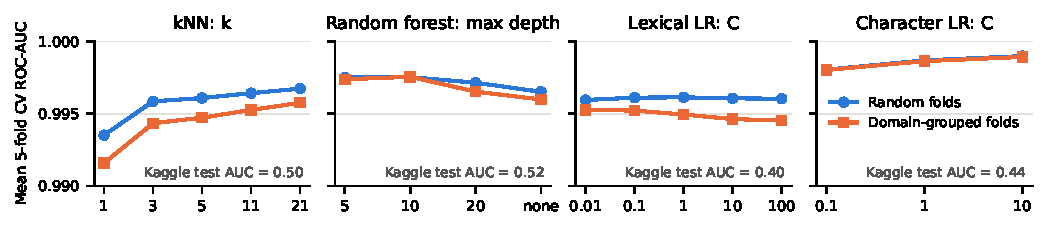
\includegraphics[width=\textwidth]{cv_roc_auc.pdf}
\vspace{-14pt}
\caption{RQ2: mean 5-fold CV ROC-AUC per hyperparameter value, with random or site-grouped folds. Grey: Kaggle test ROC-AUC of the CV-picked model.}\label{fig:cv}
\end{figure*}

\section{Results and Discussion}
\textbf{RQ1 (Table~\ref{tab:results}).} Inside PhiUSIIL the split type barely matters: all models keep ROC-AUC $\ge$0.995 and F1 $\ge$0.987, and domain-disjoint scores are even slightly higher than random. Domain grouping did not materially reduce performance on PhiUSIIL, likely because it has only 1.34 URLs per site, leaving little overlap to remove. On Kaggle all models fail. Character LR, which had the highest reported ROC-AUC on each PhiUSIIL split, goes from 24,451 TP, 269 FP, 90 FN, 26,625 TN (domain-disjoint) to 76,325 TP, 351,774 FP, 29 FN, 2 TN: it calls almost everything phishing, so precision equals the phishing share (0.178). The ranking did not carry over.

\textbf{RQ2 (Figure~\ref{fig:cv}).} The hyperparameter changes CV ROC-AUC by less than 0.005 for every model. Grouping folds by site lowers scores slightly, most for kNN with $k=1$ (0.9935 to 0.9916), which copies its nearest training URL; the picked values barely change. The grey numbers show the real problem: CV on PhiUSIIL predicted 0.996--0.999 for the picked models, but Kaggle gave 0.40--0.52. CV can only find problems inside the development data.

\textbf{RQ3 (why).} The cleaned-URL run was planned in advance (it uses the URL cleaning option from Milestone 3); the format rule is an exploratory follow-up added after the first Kaggle results. All tuning used PhiUSIIL only. The rule scores F1 0.994 with zero false alarms on the PhiUSIIL domain-disjoint test, matching or beating every trained model's F1. This suggests the models mostly learned how PhiUSIIL was built: safe means ``bare \texttt{https://www.} homepage'', which features like URL length, path length, slash count, and the HTTPS flag can pick up. Safe Kaggle URLs never look like that, so they look like phishing, and the rule fails the same way (FPR 1.000). Removing the scheme and \texttt{www.} lowers FPR only to 0.76--0.90, because paths remain. AUCs below 0.5 (e.g., Lexical LR 0.404) mean the learned cues point the wrong way on Kaggle. Near-perfect PhiUSIIL scores measure URL format, not phishing.

\textbf{Reproducibility.} \texttt{scripts/run\_evaluation.py} reruns everything (about 50 minutes on 2 CPUs); the datasets match our audit counts. Two full runs gave identical result tables (6 decimals), and 21 tests pass.

\smallskip\noindent\textbf{AI use (level D).} Claude~\cite{claude} helped write the evaluation code, figure, and draft text. We checked every number, reference, and rerun; review caught one AI bug (site names taken from cleaned URLs).

\smallskip\noindent\textbf{Team contributions.} \emph{Prabhnoor}: datasets, cross-source split, repository. \emph{Divraj}: baselines, grids, threshold. \emph{Dilraj}: CV pipeline, figure, format-rule analysis. \emph{All}: discussion, writing.

\bibliographystyle{ACM-Reference-Format}
\bibliography{references}
\end{document}
